\part{PENSAMENTO LEAN}

\chapter[Pensamento Lean]{Pensamento Lean}



\section[Lean na Manufatura]{Lean na Manufatura}

\subsection[Histórico]{Histórico}

Lean é um modo de pensar sobre como entregar valor ao cliente mais rapidamente por meio da eliminação de desperdícios que impedem a qualidade e a produtividade. O Pensamento Lean teve origem no sistema de produção da Toyota (TPS – Toyota Production System) como Lean Manufacturing e surgiu com o objetivo de reduzir desperdícios na produção. É uma filosofia de gestão que promove formas de especificar valor para o cliente, melhora sequência de fluxos de processos, torna o desempenho mais eficiente e elimina desperdícios na produção. 

Para entendermos porque e como surgiu o pensamento Lean é preciso entender o que ele substituiu: a produção em massa.  A produção em massa foi popularizada por Henry Ford. A produção em massa é usada para produzir em larga escala a baixo custo. Ela divide o processo de manufatura em pequenos passos que possam ser desempenhados por trabalhadores com poucas habilidades, para isso é usado um maquinário de alta precisão e um trabalho padronizado. A produção em massa tem uma característica de inflexibilidade, pois alterações na linha de produção podem acarretar alto custo, assim, apenas é econômico produzir grandes quantidades da mesma coisa e da mesma forma (padronização) \cite{hibbs2009}. 

Em 1945, no Japão pós-guerra, o presidente da Toyota Motor Company, Kiichiro Toyoda, desafio sua companhia a se igualar às companhias da América, porque se não a indústria automobilistica Japonesa não sobreviveria. E ficou claro que isso não poderia ser feito adotando o modelo de produção em massa norte-americano, pois no Japão os materiais eram escassos, as encomendas eram inconstantes e havia demanda por variedade, o que impediria o sucesso de produção larga escala de produtos idênticos. 

Taiichi Ohno, chefe de produção da Toyota, notou essas características que inviabilizam a indústria automobilistica japonesa de adotar o modelo de produção em massa. Com isso, Taiichi Ohno experimentou muitas ideias e técnicas que foram inseridas aos poucos no que veio a ser conhecido como Sistema Toyota de Produção. Ele estudou o sistema de produção de Henry Ford e ampliou sua visão como os supermercados norte-americanos controlavam seus estoques. E acrescentou seus conhecimentos de fiação e tecelagem e as percepções dos trabalhodores que ele supervisionava. Ele descreveu o sistema como “um sistema para absoluta eliminação de desperdícios” e explica que o sistema se mantém sobre dois pilares: Just-in-Time (JIT) e Jidoka (autonomação). 

O fluxo Just-in-Time é o único modelo industrial para gerenciar com eficiência a complexidade inerente do custo de se produzir com variedade. Durante muitos anos o Sistema Toyota de produção foi ignorado, até mesmo no Japão, no entanto, após a crise econômica do petróleo nos anos 70, o sistema foi estudado e adotado por outras empresas japonesas devido ao fato de a Toyota ter emergido da crise rapidamente. Após uma década, o Japão passou a ser forte concorrente dos Estados Unidos e da Europa. Com uma investigação, foi descoberto que as empresas japonesas estavam utilizando uma nova abordagem chamada Just-in-Time, que diz respeito ao princípio de eliminar estoques que costuma estarem presentes em produção de larga escala, tendo o foco em fazer tudo em pequenos lotes e estar apto a realizar mudanças de forma rápida. 

O Jidoka surgiu como o mecanismo utilizado pela máquina de tear automática G-Type criada por Kiichiro, ele consiste na paragem automatica da máquina quando um fio quebrava, evitando que ocorressem desperdícios de material ao se produzir produtos defeituosos. Ao eliminar a criação de produtos defeituosos e diminuir desperdícios no processo, a máquina se tornou um sucesso absoluto, melhorando tanto a produtividade quanto a eficiência do trabalho \cite{katayama2010}. Com isso, o conceito que ficou com o Jidoka foi: organizar o trabalho de modo que ele seja imediatamente interropido quando a menor anomalia for detectada, sendo necessário encontrar a causa e a resolução do problema antes de recomeçar a atividade. No português, Jidoka significa autonomoção, que diz respeito ao fato de responder aos eventos de forma instantânea e correta sem ter que ir ao cérebro receber instruções, no caso da máquina assim que surgir um problema ela para \cite{poppendieck}. 

O sistema de produção sofreu alterações ao longo das décadas, nos anos 90 o Pensamento Lean passou a ser o termo usado para descrever este processo desenvolvido e utilizado pela Toyota. Assim, o Sistema Toyota de Produção, baseado no que hoje é chamado de Pensamento Lean, começou a ser formado nos anos 50 e aos poucos os resultados puderam ser notados na indústria automobilistica mundial. Como a figura 4 mostra nos anos 50 a Toyota nem sequer aparecia do ranking de vendas liderado pela GM e pela Ford. Já nos anos 70 o cenário começou a mudar, a Toyota passou a aparecer na sexta posição do ranking e teve uma ascendência até 2007 onde se tornou líder do ranking de vendas.

\begin{figure}[h]
		\centering
		\label{fig01}
			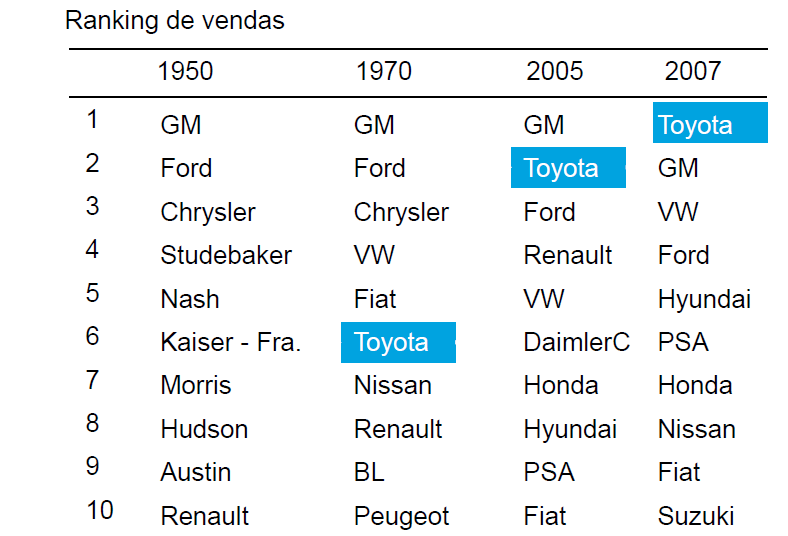
\includegraphics[scale=0.5]{figuras/ranking.png}
		\caption{Ranking de Vendas da Indústria Automobilística  \cite{ranking}}
\end{figure}

\subsection[Princípios]{Princípios}

O Pensamento tem como objetivo fornecer o que o cliente deseja sem haver desperdícios. Para atingir este objetivo Lean possui alguns princípios. Muitas companhias e indivíduos que querem implementar o Pensamento Lean cometem o erro de ficarem preocupados e focados em especificar ferramentas e práticas. Quando aplicadas de forma correta, as ferramentas podem gerar bons resultados de desempenho, mas são os princípios inseridos na cultura da organização que resultarão na mudança de comportamento em longo prazo. Sem uma clara compreensão dos princípios que regem o Pensamento Lean, as empresas conseguirão resultados a curto prazo, mas a longo prazo não consiguiram manter esses bons resultados e a melhoria contínua que irão dar estabilidade ao negocio e à satisfação do cliente. Assim, é preciso enfativar os princípios acima das ferramentas. 

\begin{figure}[h]
		\centering
		\label{fig02}
			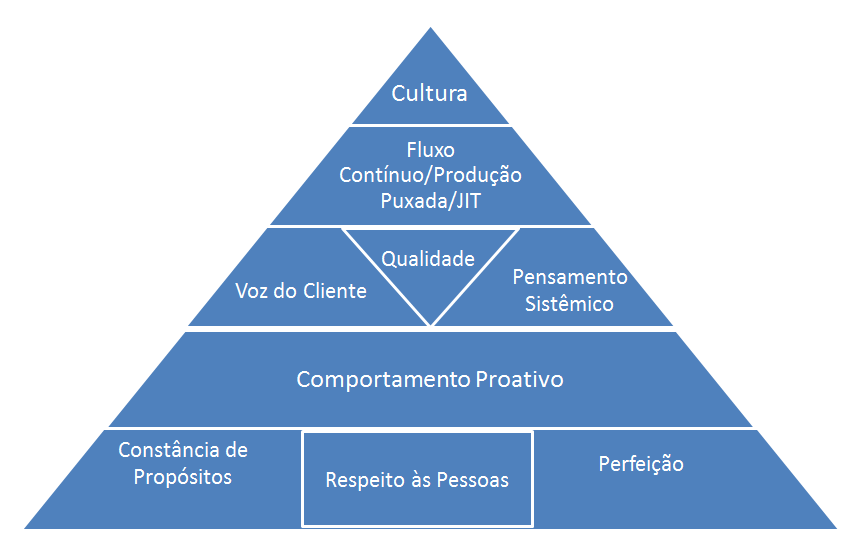
\includegraphics[scale=0.7]{figuras/principioslean.png}
		\caption{Pirâmide de Princípios Lean}
\end{figure}

Os princípios do Pensamento Lean na Manufatura são apresentados na figura 5. Tais princípios são usados como base para a definição dos princípios e práticas do Lean no Desenvolvimento de Software que serão apresentados na seção a seguir. Os detalhes sobre no que consiste cada um dos princípios, práticas e ferramentas do Lean na Manufatura podem ser encontrados no Anexo B - Princípios e Práticas Lean na Manufatura.

\section[Lean no Desenvolvimento de Software]{Lean no Desenvolvimento de Software}

\subsection[Abordagem]{Abordagem}

Mary e Tom Poppendieck fizeram um mapeamento dos princípios Lean na Manufatura em sete princípios em Lean no Desenvolvimento de software. Tais princípios serão detalhados nas seções a seguir. 

\subsection[Princípios]{Princípios}

\subsubsection[Eliminar o Desperdício]{Eliminar o Desperdício}

Eliminar desperdícios no sistema Lean de produção (manufatura) funciona da seguinte forma: olhar a linha do tempo desde a concepção do produto até a entrega ao cliente, e remover aquilo que não acrescenta valor (desperdícios). No desenvolvimento Lean de software o objetivo de eliminar desperdícos é o mesmo, porém, o início e  fim da linha do tempo podem ser alterados. A linha do tempo no desenvolvimento de software tem início no momento do pedido e para quando o pedido é entregue. Reduzir os desperdícios na linha do tempo significa reduzir a própria linha do tempo, ou seja, entregar o que foi pedido o mais rápido possível e com qualidade  \cite{poppendieck}.

Para conseguir eliminar desperdícios é preciso, primeiramente, identificá-lo. Como desperdício é tudo que não agrega valor, é preciso ter conhecimento do que realmente é o valor. Na área de desenvolvimento de software, identicar o que é valor para o cliente é algo mais complexo, pois, dificilmente, no início do desenvolvimento o cliente sabe realmente o que quer, as suas necessidades e os seus desejos mudam ao longo do desenvolvimento, alterando a definição do que agrega valor. No entanto, grandes organizações têm conseguido ter um conhecimento profundo do que é valor para o cliente e têm conseguido satisfazer suas necessidades. Assim, o objetivo de todas as organizações é conseguir alcançar esse entendimento profundo de valor.

A partir do momento que as pessoas conseguem identificar o que é valor, é possível começar a desenvolver a capacidade de identificar o que é desperdício. Qualquer atividade, não importante, que impeça o cliente de receber o que ele deseja e quando ele deseja é desperdício. Semelhante ao estoque no sistema produtivo, trabalhos inacabados no desenvolvimento de software gera todos os prejuízos com o fato de ser perdido, estar tecnologicamente atrasado, esconder problemas de qualidade e estagnar dinheiro.

Especificamente no desenvolvimento de software alguns desperdícios acontecem de forma constante: todos os requisistos especificados no início, que obviamente irão sofrer mudanças, testes realizados muito perto do fim, que claramente vão gerar muito retrabalho, e principalmente, funcionalidades desenvolvidas que nunca chegam a ser utilizadas.  De fato, estima-se que cerca de 20% das funcionalidades em um sisstema personalizado são regularmente usadas e cerca de dois terços delas são raramente usadas, o que gera custos desnecessários. 

\subsubsection[Integrar Qualidade]{Integrar Qualidade}

A meta dentro do desenvolvimento de software Lean é construir software com qualidade desde o início, não deixar para inserir testes só no final do de senvolvimento. A organização precisa ser bastante disciplinada. Para desenvolver um software com qualidade é preciso controlar as condições desde o começo de forma a não permitir defeitos. Como não é possível previnir todos os defeitos, é indicado inspecionar o produto após cada pequena funcionalidade ser implementada para que possa encontrar o defeito imediatamente após surgirem \cite{poppendieck}.

É importante ressaltar que o slogan “faça certo na primeira vez”, muito comumente usado, não se refere a construir o código e jamais modificá-lo, mas sim ao fato de usar-se as técnicas Test Driven Development (TDD), integração contínua e refatoração para garantir que um código simples e limpo que agregue valor ao cliente. 

\subsubsection[Criar Conhecimento]{Criar Conhecimento}

O desenvolvimento de software é um processo de criação do conhecimento.  Um processo de desenvolvimento concentrado em criar conhecimento esperará que o projeto evolua durante a codificação e não desperdiçará muito tempo fazendo todos os requisitos e arquitetura prematuramente. 

As empresas que já mostraram uma excelência a longo prazo em desenvolvimento de produtos compartilham um traço em comum: elas geram novo conhecimento por meio de uma experimentação disciplinada e codificam este conhecimento concisamente para torná-lo acessível ao restante da organização. Essas empresas não somente capturam dados explícitos, mas encontram maneiras de tornar explícito o conhecimento tático e fazê-lo parte da base de conhecimento organizacional \cite{nonaka}.

É importante ter um processo de desenvolvimento que encoraje o aprendizado sistemático durante todo o ciclo de desenvolvimento e também é preciso melhorar os processos de desenvolvimento continuamente. Às vezes, na constante busca por padrões ou modelos de processos, as empresas se prendem a uma documentação que torna mais difícil para as equipes de desenvolvimento reservar um tempo para melhorar diariamente seus próprios processos. Em Lean devem-se melhorar continuamente os processos, pois em ambientes complexos sempre haverão problemas. Assim, para cada problema é preciso acionar uma busca pela causa raiz, construir soluções possíveis para o problema e acionar uma mudança no processo para impedir que o problema ressurja \cite{poppendieck}. 

\subsubsection[Adiar Comprometimentos]{Adiar Comprometimentos}

A ideia principal deste princípio é deixar as decisões irreversíveis para o último momento possível, ou seja, a última oportunidade de tomar a decisão antes que seja tarde demais, afinal de contas uma tomada de decisão é um compromisso que é firmado. Porém, isto não quer dizer que todas as decisões devam ser adiadas. Em primeiro lugar, é preciso tentar tornar a maioria das decisões reversíveis, ou seja, que possam ser mudadas ao decorrer do desenvolvimento sem prejuízos significativos. Um sistema de software não precisa ser completamente flexível, mas precisa que opções sejam preservadas em pontos onde as mudanças invariavelmente ocorram. É preciso experiência para saber quando devem ser mantidas essas opções  \cite{poppendieck}.

\subsubsection[Entregar Rápido]{Entregar Rápido}

A ideia deste principio é que é preciso entregar o software tão rápido que os clientes não tenham tempo de mudar de ideia.  As empresas que competem com base no tempo frequentemente têm uma vantagem significativa de custo sobre seus concorrentes. E para isso ser possível, elas eliminaram uma grande quantidade de desperdício, e desperdício tem influência diretamente no prazo e no custo. Além disso, velocidade repetível e confiável não é possível sem desenvolver com grande qualidade e, ainda, para ter sucesso tais empresas desenvolveram um profundo conhecimento sobre o que é valor para o cliente. Com a rapidez, é possível testar novas ideias e aprender o que funciona ou não funciona  \cite{poppendieck}. 

\subsubsection[Respeitar as Pessoas]{Respeitar as Pessoas}

O princípio de respeitar as pessoas diz respeito a não impedir que as pessoas façam seus trabalhos só porque um outra pessoa acredita que não é a melhor forma de fazê-lo. Todos devem respeitar-se e trabalharem juntos na melhor solução. No processo de desenvolvimento também deve haver respeito, todos devem fazer parte da melhoria contínua dos processos. Existem três bases que sustentam o respeito às pessoas  \cite{poppendieck}:

\begin{itemize}
\item Líder empresarial: uma empresa que respeita as pessoas desenvolve bons líderes e garante que a equipe tenha o tipo de liderança que promove pessoas engajadas e pensantes, concentrando seus esforços na criação de um ótimo produto.
\item Mão de obra técnica especializada: empresas sábias garantem que a especialização técnica apropriada seja estimulada dentro da própria empresa e que as equipes estejam abastecidas da especialização necessária para atingir determinado objetivo.
\item Responsabilidade baseada em planejamento e controle: respeitar as pessoas significa que as equipes recebem planos genéricos e objetivos claros, e em vez de dizer como e o que fazer, desenvolve uma organização reflexiva onde as pessoas usam suas cabeças e descobrem isso sozinhas.
\end{itemize}

\subsubsection[Otimizar o Todo]{Otimizar o Todo}

Uma organização Lean otimiza todo o fluxo de valor, do momento em que recebe o pedido visando uma necessidade do cliente até o momento em que o software seja implantado e a necessidade do cliente seja atendida. Se houver concentração em otimizar apenas uma pequena parte do todo, inevitavelmente, o fluxo de valor completo sofrerá. 

\subsection[ Práticas]{ Práticas}

\subsubsection[Gerenciamento de Código Fonte e Scripts de Builds]{Gerenciamento de Código Fonte e Scripts de Builds}

O Gerenciamento de Código Fonte e Scripts de Builds não são práticas exclusivas do Lean, mas sim uma prática que deveria ser usada adotando Lean ou não, por isso é considerada como um pré-requisito para as práticas do Lean. Estas práticas ajudam a construir um time disciplinado e um ambiente de desenvolvimento estável.

O Gerenciamento de Código Fonte também é conhecido como controle de versão, basicamente, diz respeito a manter todo o código fonte e outros artefatos importantes do projeto em um repositório que mantém um histórico de versões de todos os itens de configuração, que são artefatos que precisam ser mantido sobre controle, pois sofrem mudanças e evoluções. Com o controle de versão é possível recuperar uma configuração, versão dos itens de configuração, em um momento desejado do tempo. Sempre é possível retornar a uma versão estável (baseline) quando erros são identificados.

O objetivo de realizar scripts de builds é automatizar todo o processo de construção do sistema e garantir que as mudanças no projeto são construídas, testadas e relatadas tão logo quanto o possível depois de serem relatadas. Como resultado, o build do sistema é gerado da mesma forma em todas as vezes. Esta prática elimina erros escondidos e torna mais fácil a inserção de novos integrantes à equipe. E também torna mais fácil realizar testes e a entrega de release do software, uma vez que constrói arquivos executáveis e de instalação do produto \cite{hibbs2009}.

\subsubsection[Teste Automatizado]{Teste Automatizado}

Um sistema à prova de erros é uma das práticas fundamentais do Lean. É parte central da produção de um produto com qualidade e da redução de desperdícios. O teste automatizado é um dos principais meios de evitar erros no desenvolvimento de software. O teste automatizado engloba todos os tipos de testes: teste unitário, teste de integração, teste de aceitação, teste de desempenho, teste de carga, desenvolvimento orientado a testes, etc.

Cada um dos tipos de testes possui um objetivo principal, mas todos eles têm os seguintes objetivos em comum:
\begin{itemize}
\item Os testes são criados manualmente pelos desenvolvedores.
\item Todos os testes podem ser executados automaticamente, sem intervenção humana.
\item Os erros são detectados automaticamente.
\item O desenvolvedor é notificado quando os erros acontecem.
\end{itemize}

O teste automatizado suporta três princípios do Lean: eliminação de desperdícios, qualidade na raiz e criar conhecimento. Ele ajuda a eliminar desperdícios que geram retrabalho e custos quando erros são detectados apenas nas fases finais do ciclo de desenvolvimento de software. No que diz respeito a construir com qualidade, o teste automatizado é um dos principais meios. Uma base de código com uma suíte de testes automatizados realiza a validação e checagem de forma automática, o que reduz a possibilidade de erros não detectados seja introduzido dentro do software.

Além disso, os testes automatizados servem como uma documentação atualizada do que está sendo feito. Ele cria um conhecimento primário e confiável para os desenvolvedores porque garante conformidade com o esperado toda vez que a suíte de teste é executada com sucesso \cite{hibbs2009}.

\subsubsection[Integração Contínua]{Integração Contínua}

A integração diz respeito ao momento que todos os módulos ou componentes do software que está sendo desenvolvido são executados juntos. Componentes individuais, banco de dados, interfaces de usuário e recursos do sistema são todos reunidos e testados em cima da arquitetura. A integração envolve verificar a comunicação dos componentes e garantir que a mensagem passada entre eles é compatível e completa. 

O processo de desenvolvimento tradicional trata integração como uma fase separada que ocorre depois que todos os componentes tenham sido implementados, o que costuma gerar uma serie de correções e retrabalho. A integração contínua transforma a tradicional fase de integração em uma atividade que ocorre durante toda o processo de implementação do sistema.

A integração contínua é o processo de integrar pequenas mudanças em uma base estável para entrega de um novo release do produto. Integrando pequenas mudanças em um curto intervalo, os desenvolvedores podem evoluir o produto um pouco de cada vez enquanto garantem que cada novo pedaço funciona corretamente com todo o resto do sistema. A integração contínua usa testes unitários para garantir que cada pequena parte do sistema está implementada corretamente e usa o gerenciamento do código fonte e os scripts de build para garantir que a cada nova pequena integração nada foi quebrado, ou seja, garantir que o sistema continue funcionando corretamente como um todo \cite{hibbs2009}. 

\subsubsection[Menos Código ]{Menos Código}

A prática de escrever menos código não diz respeito a escrever menos software, mas sim a ter todas as funcionalidades implementadas com poucas linhas de código e de maneira simples. Diz respeito a eliminar código desnecessário e fazer com que o código necessário se torne mais eficiente, mantendo a base de código pequena ao menos tempo em que funcionalidades (valor) são entregues ao cliente.

O tamanho da base de código afeta o projeto de vários modos. Quanto maior o código maior é a quantidade de componentes que precisam ser conectadas e mais esforço de integração será gasto. Quanto maior o tamanho da base de código mais erros podem ser gerados e mais esforço para encontrar e corrigir os erros será gasto. Ainda, quanto maior o tamanho maior é a dificuldade de entender o que foi desenvolvido, aumentando a curva de aprendizado de novos desenvolvedores e futuros mantedores.  

Como uma base de código grande acarreta em mais componentes, mais bugs e grande curva de aprendizagem, como consequência terá mais custos em desenvolvimento e manutenção. A definição de desperdício no desenvolvimento Lean é qualquer coisa que aumente os custos sem produzir valor, então o custo de desenvolvimento e manutenção resultante de uma grande base de código pode ser considerado como desperdício. 

Para escrever menos código e manter o valor desejado pelo cliente, os desenvolvedores precisam adotar uma atitude de olhar criticamente para cada linha de código. Minimizar o tamanho do código, no entanto, não é limitar a implementação. Os desenvolvedores precisam ser minimalistas durante todo o processo de desenvolvimento, desenvolvendo de maneira simples cada funcionalidade. Um design simplista facilita, ainda, a implementação de mudanças \cite{hibbs2009}. Os padrões e técnicas podem ser utilizados para auxiliar os desenvolvedores a desenvolver apenas o código que é realmente necessário, por exemplo, utilizar padrões de design, reuso e refatoração.

\subsubsection[Iterações Curtas]{Iterações Curtas}

O desenvolvimento iterativo entrega software funcional ao cliente para avaliação a cada intervalo específico de tempo. Cada iteração adiciona novas funcionalidades ao produto e aumenta o entendimento do cliente sobre como o produto final irá atender à suas necessidades. A efetividade do processo iterativo vem da oportunidade de ter o feedback do cliente e incorporar esse feedback ao desenvolvimento. O feedback do cliente é que irá direcionar a próxima iteração quanto a adição, remoção ou modificação de requisitos e implementação. Quanto menor a iteração, mais oportunidades de receber o feedback do cliente e maior é a possibilidade de atender o que o cliente deseja no produto final. 

As iterações curtas suportam três princípios do Lean: eliminar desperdício, adiar compromisso e entrega rápida. Existem duas formas de desperdícios advindos de iterações largas, o trabalho parcial, aquele que não é construído de forma completa seja com requisitos não implementados ou incompletos quanto com código não testado, porque não adiciona novo valor ao produto e o replanejamento, quando o planejamento inicial é feito para um futuro muito distante e as necessidades e desejos do cliente podem mudar fazendo com que seja preciso o realizar o replanejamento, porque o trabalho planejado anteriormente é desperdiçado. As iterações curtas previnem tais situações de desperdícios, pois o esforço fica concentrado em desenvolver o que é de alta prioridade para o cliente mais rapidamente e planeja tão longe quanto necessário para manter o desenvolvimento.  

O princípio de adiar compromisso, como já explicado anteriormente, diz respeito a adiar decisões importantes tanto quanto possível. Adiar tais decisões fornece aos desenvolvedores tempo para coletar e entender as informações necessárias para o desenvolvimento, e iterações curtas dão oportunidades de coletar informações por meio do feedback do cliente. Os desenvolvedores podem criar protótipos do produto final já nas iterações iniciais, recebem o feedback e usam o feedback para decidir a implementação final nas iterações finais \cite{hibbs2009}.

As iterações curtas, claramente, suportam o princípio de entrega rápida devido a redução dos intervalos de contato com o cliente e por entregar novas funcionalidades rapidamente para receber feedback. Em vez de esperar até o final do desenvolvimento para vê os efeitos das suas solicitações, o cliente já poderá visualizá-los na próxima iteração. 

\subsubsection[Participação do Cliente]{Participação do Cliente}

Se o objetivo do desenvolvimento de um produto é criar um produto que o cliente irá usar, é importante ter a participação do cliente em grande parte do processo. Os conceitos de priorizar requisitos e de realizar correções de acordo com o feedback do cliente necessitam de participação ativa do cliente no processo de desenvolvimento. 
Os clientes são as melhores fontes de informações sobre o domínio do problema.  Eles sabem as atividades que precisam ser feitas, eles sabem as condições que o software será executado e eles sabem os objetivos que desejam atingir com a solução. No entanto, eles raramente sabem sobre a tecnologia que será usada na implementação da solução.  

Por outro lado, os desenvolvedores sabem sobre as a tecnologias e sabem o caminho mais eficiente para modelar e implementar problemas e soluções. O que os desenvolvedores não sabem é sobre os conhecimentos do negócio no qual a solução será incorporada. 

Combinando o conhecimento do negócio do cliente com o conhecimento técnico do desenvolvedor cria uma equipe dinâmica que resulta em um desenvolvimento de um melhor produto. Desenvolvedor e clientes trabalhando juntos inspiram um ao outro a criar algo melhor do que eles poderiam criar individualmente \cite{hibbs2009}.


\subsubsection[Kanban]{Kanban}

O Kanban no desenvolvimento de software surgiu a partir do Kanban do Lean na manufatura, ambos usam um mecanismo de controle visual para acompanhar o trabalho à medida que ele flui através das várias etapas do fluxo de valor. 

\begin{figure}[h]
		\centering
		\label{fig05}
			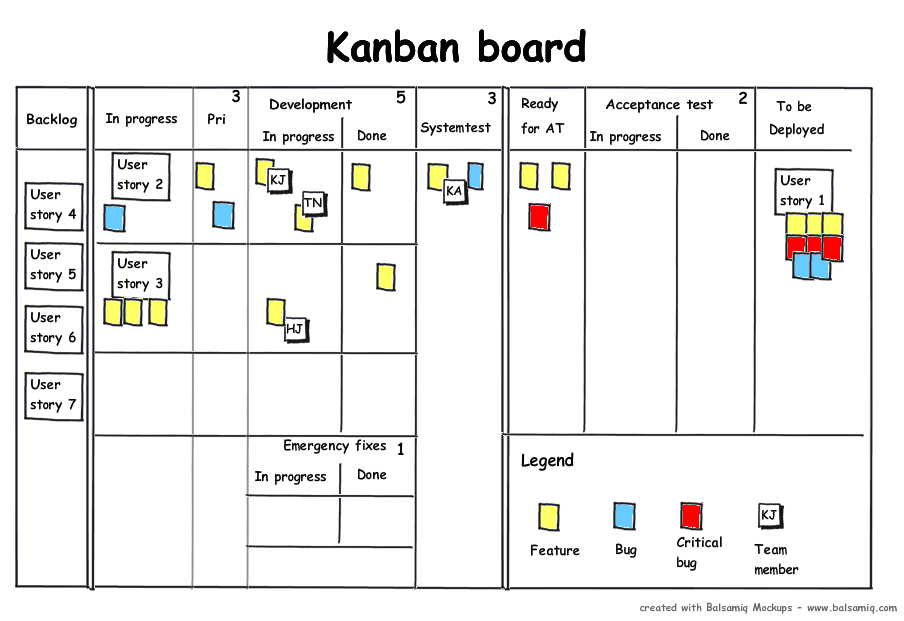
\includegraphics[scale=0.7]{figuras/kanban.png}
		\caption{Quadro Kanban \cite{kanban}}
\end{figure}

O Kanban não é um processo ou ciclo de vida de gerenciamento de projetos ou de desenvolvimento de software. Ele é uma abordagem para introduzir mudanças em um ciclo de desenvolvimento de software ou metodologia de gerenciamento de projetos. O Kanban tem três conceitos básicos: visualizar o fluxo de trabalho, limitar o trabalho em progresso (WIP – work in progress) e medir e melhorar o fluxo \cite{kniberg2009}. 

Para visualizar o fluxo de trabalho divida o trabalho em partes, escreva cada item em um cartão, ou post-its, e coloque no quadro Kanban, e use colunas nomeadas para ilustrar onde cada item está no fluxo de trabalho. Com o mapeamento do fluxo de trabalho já é possível ter o entendimento do processo atual. 
Para limitar o WIP é preciso associar limites explícitos para quantos itens podem estar em progresso em cada estado do fluxo de trabalho, existe um número limite de tarefas que podem ser bem feitas durante um mesmo período de tempo \cite{klipp}. 

É preciso saber também a diferença entre a complexidade das tarefas, duas tarefas podem ser feitas em uma semana assim como duas tarefas podem ser feitas em três horas, tudo dependerá de quanto esforço será gasto em cada uma. As métricas do Kanban ajudam a chegar a um número ótimo.

\begin{figure}[h]
		\centering
		\label{fig05}
			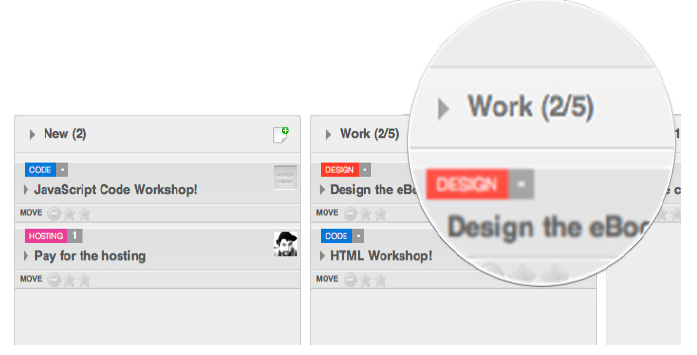
\includegraphics[scale=0.5]{figuras/WIP.png}
		\caption{Work in Progress  \cite{klipp}}
\end{figure}


Além disso, com o WIP limitado em um sistema Kanban, tudo que fica bloqueado por qualquer motivo tende a parar o sistema. Se certa quantidade de itens de trabalho fica bloqueada, todo o processo para de funcionar. Isso cria a necessidade de concentrar toda a equipe e toda a empresa na solução do problema para desbloquear o item e restaurar o fluxo. 

A melhoria deve sempre ser baseada em objetivos mensuráveis, e no Kanban isto não é diferente. Encontrar e aplicar boas métricas é geralmente um passo difícil,  mas algumas métricas simples automaticamente geradas por uma aplicação pode dar a informação necessária para otimizar o processo e maximizar a eficiência \cite{klipp}. 

\begin{figure}[h]
		\centering
		\label{fig05}
			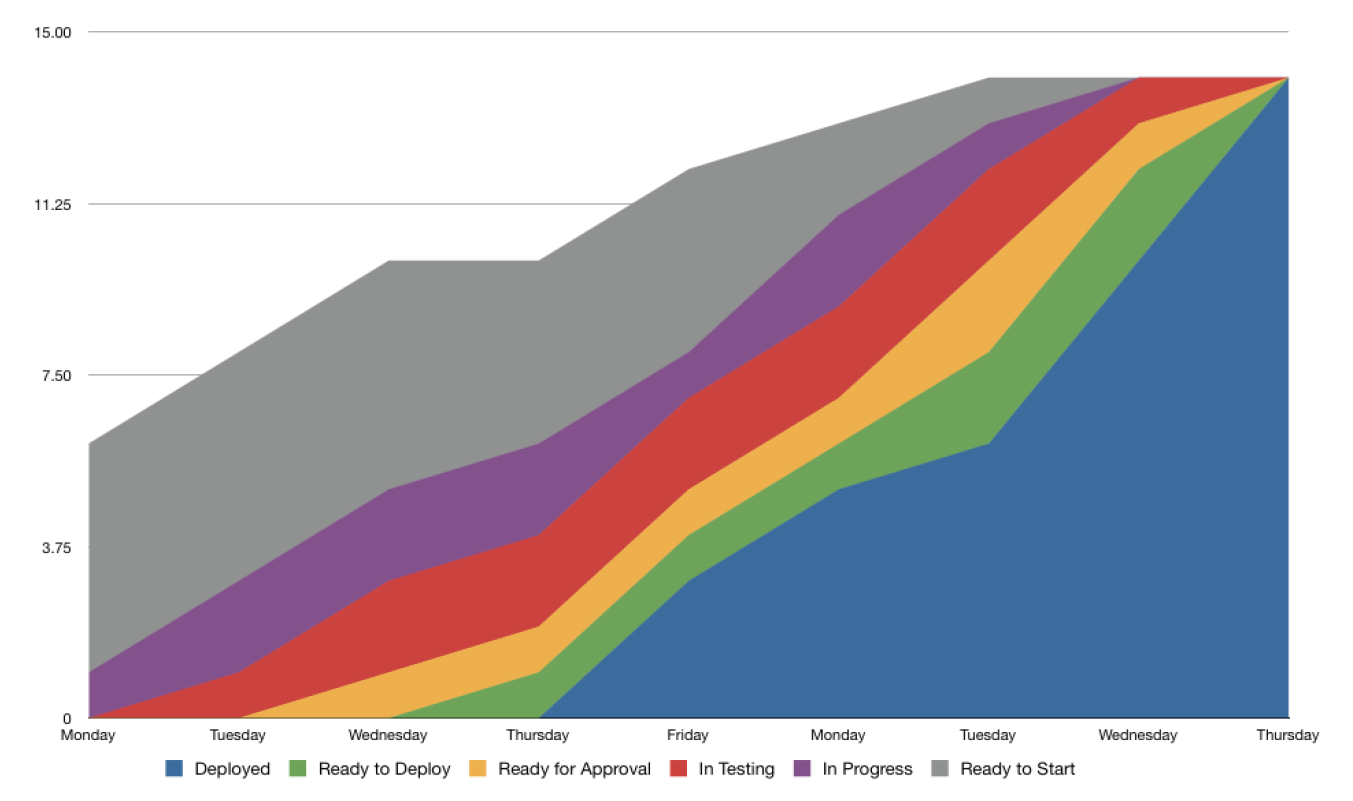
\includegraphics[scale=0.4]{figuras/metricasKanban.png}
		\caption{Gráfico de Medições Kanban  \cite{klipp}}
\end{figure}

O Kanban, no entanto, vai um passo além e dá transparência ao processo e seu fluxo. O Kanban expõe gargalos, filas, variabilidade e desperdício. Tudo que impacta o desempenho da organização em termos de quantidade de trabalho de valor entregue e o tempo de ciclo necessário para entregá-lo. Proporciona aos membros da equipe e às partes interessadas externas a visibilidade sobre os efeitos de suas ações (ou falta de ações) e esta visibilidade incentiva a discussão sobre melhorias que precisam ser feitas nos seus processos encorajando a evolução incremental dos processos existentes. Ainda, o  Kanban, através da natureza do sistema pull, encoraja também comprometimento tardio, tanto em priorização de trabalho novo quanto na entrega de trabalho existente \cite{kniberg2009}. 
